\documentclass[12pt]{article}
\usepackage{geometry}
\usepackage{booktabs}
%-----------------------------format.tex-----------------
\usepackage{amsmath,amssymb}
\usepackage{graphicx}
\usepackage{fancybox}
\usepackage{fancyhdr}
\usepackage{float}
\usepackage{lastpage}
\usepackage{hyperref}
\hypersetup{
    unicode={true},pdfstartview={FitH},pdfborder={0 0 0},
    colorlinks,linkcolor=blue,citecolor=blue,hyperindex,plainpages=false,}
% style: page layout
\setlength{\headheight}{15pt}
\setlength{\headsep}{20pt}
\setlength{\footskip}{30pt}
\setlength{\voffset}{-5pt}
\setlength{\hoffset}{16pt}
\setlength{\oddsidemargin}{0pt}
\setlength{\evensidemargin}{\oddsidemargin}
\setlength{\marginparpush}{0pt}
\setlength{\marginparwidth}{0pt}
\addtolength{\textheight}{3\baselineskip}
\hypersetup{
	colorlinks=true,
	linkcolor=black
}
\newtheorem{definition}{{definition}}
\newcounter{numdefinition}
\renewenvironment{definition}[1]
{\noindent\stepcounter{numdefinition}
\slshape Definition \arabic{numdefinition} \textsf{#1 :}
\begin{quote}\small\itshape}
{\end{quote}}

\newcommand{\dd}{\ensuremath{\,\mathrm{d}}}
%===============================================================
\fancypagestyle{plain}%���¶���plain��ʽ,����summary sheet
{\fancyhf{}
\setlength{\headheight}{0pt}\setlength{\headsep}{0pt}
\setlength{\voffset}{-50pt}\setlength{\oddsidemargin}{0pt}}

\graphicspath{{pic/}}
%=========================����ҳü===============================
\pagestyle{fancy} 
\rhead{page \thepage\ of \pageref{LastPage}}
\chead{} \lhead{Team \footnotesize{\#} 201906177} \lfoot{}
\cfoot{\thepage}
\rfoot{}
\renewcommand{\headrulewidth}{0.4pt}

\begin{document}

%=========================summary sheet.tex========================

\thispagestyle{empty}
\begin{minipage}{0.3\textwidth}
%\begin{flushleft}
%For office use only\\
%   T1\ \rule{3cm}{0.5pt}\\
%   T2\ \rule{3cm}{0.5pt}\\
%   T3\ \rule{3cm}{0.5pt}\\
%   T4\ \rule{3cm}{0.5pt}\\
%\end{flushleft}
\end{minipage}\hspace{\fill}
\begin{minipage}{0.3\textwidth}
\centering
Team Control Number\\[5pt]
\fontsize{20pt}{\baselineskip}\selectfont  \textbf{201906177} \normalsize\\[10pt]
Problem Chosen\\[5pt]
\fontsize{18pt}{\baselineskip}\selectfont \textbf{A }\normalsize\\
\end{minipage}\hfill
\begin{minipage}{0.35\textwidth}
%\begin{flushright}
%\shortstack[l]{
%For office use only\\
%   F1\ \rule{3cm}{0.5pt}\\
%   F2\ \rule{3cm}{0.5pt}\\
%   F3\ \rule{3cm}{0.5pt}\\
%   F4\ \rule{3cm}{0.5pt}}
%\end{flushright}
\end{minipage}\vspace*{10pt}
\rule{\textwidth}{0.5pt}

\begin{center}
  \textbf{ShuWei Cup}
\end{center}
%\enlargethispage
\noindent
{\Large \textbf{Summary}}
\vspace{7pt}

%==========================abstract.tex================================

In view of the first problem, on the basis of the traditional grey prediction model, the Markov chain is used to correct the prediction result error, and the grey Markov model is obtained and predicted. This group first established the traditional GM (1,1) model to predict and analyze the number of elderly people and medical needs in the period of 2009-2021. Then through Markov model, the expected value of predicted residual is calculated. Finally, residual expectation is used to correct the inherent deviation of traditional grey prediction. The prediction error of the model is less than 7\%, and the NSE value approaches to 1, which indicates that the model has high reliability.
~\\

To solve the problem two, the problem based model was used to predict the characteristics of the disease, and then the key prevention and control objects were selected by TOPSIS. Firstly, the number of disease and death in Hubei Province is selected into the grey Markov model of question one. The number of morbidity and mortality, the growth rate of morbidity and mortality and the morbidity and mortality in 2019-2021 are predicted. The above five indexes are brought into the TOPSIS comprehensive evaluation model, with weights of 0.15, 0.3, 0.15, 0.3 and 0.1 respectively. The comprehensive evaluation scores of each population and each region are calculated. The ranking results show that heart disease is the key monitored disease in Hubei Province.

~\\

\textbf{keyword}: GM (1,1); Markov; TOPSIS;%xxx speed; finite element method; 
\newpage

%====================Ŀ¼ҳ========================================
\thispagestyle{empty}
\setcounter{page}{0}
{\begin{center}\Large \textbf{}\end{center}}
\tableofcontents                                                  %
\newpage                                                          %
%==================================================================

\newcommand{\vw}{\frac{v_i}{\omega_i}}

%=======================\input{introduction1}=======================

\section{Introduction}	
\subsection{Background}

	With the rapid development of China's economy and the deepening trend of aging, people's demand for hospital health services is also getting higher and higher. Therefore, it is of great significance to establish an appropriate model to study the trend of aging in the future and the trend of people's demand for medical care. At the same time, the establishment of a reasonable competition and cooperation mechanism between private and public hospitals can also maximize the utilization of resources.

\subsection{Work}
	The problem requires us to make rational use of network resources?answer the following questions
	
	\begin{itemize}                                             
		\item [1.] The aging trend of China and the people's medical needs to make a reasonable forecast.
		\item [2.] Take a province as an example to analyze the most common disease in the future.
		\item [3.] According to the medical needs of patients, an optimal queuing method is proposed to equalize the number of queues between different hospitals and different departments of the same hospital.
		\item [4.] Put forward the best cooperation and competition strategy between private hospital and public hospital.
		\item [5.] Write recommendations for relevant medical departments and prepare "14 five-year plans" for their reference.
	\end{itemize}		

%============================\input{definitions1}===========
\section{Problem Analysis}
\paragraph{Analysis of task one}


According to the relevant data from 2009 to 2018 in the National Bureau of statistics, the group first selects appropriate indicators and then establishes a grey prediction model to predict and analyze the population aging trend and residents' medical needs of the epidemic in 2009-2018. Then, through the Markov model, the data from 2009-2018 simulates the distribution of residual in each interval and calculates the expectation of the predicted residual in 2019-2021 Value. Finally, the prediction results and residual expectation are made to be different, and the inherent deviation of traditional grey prediction is corrected. Through the combination of the two models, the goal of scientific prediction of the future development of population aging and the trend of residents' medical needs is achieved. 


\paragraph{Analysis of task two}

According to the second question, we are asked to analyze the most common diseases in a specific province in the future . we took the Hubei province as an example to collect data on common diseases such as heart  disease ,and established a model with Markov model.And calculated The number of cases, growth rate of cases, growth rate of deaths and death rate of each disease ,Then substituted the five index data into the principal component analysis model. The disease with the highest score was the most common disease in the province in the future.

\paragraph{Analysis of task three} 
The task three ask us to propose a common queuing theory method and figure its related optimal queuing for this kind of queuing problem.Via refering to the operational mode of the real world hospital, we choose to adopt the $M/M/c/\infty$ model as the required theory. Then we acquire the hospital statistics and abstract the data into the parameter in model. Finally, to get the social cost to be lowest, we manage to find the optimized systems design for the queuing model.

\paragraph{Analysis of task four}
The task four ask us to analyse the complex cooperation and competition between private hospitals and public hospitals then propose the optimal cooperation and competition strategies among multiple hospitals. After refering to a deal of data and document, we are aware of that there exist complicated partnerships. Based on latent class analysis (LCA),we would provide the best strategies we come up with. 
%\paragraph{Analysis of task five}
%=======================\input{Assumptions1}=====================================
	\section{Symbol and Assumptions}
\subsection{Symbol Description}
\begin{center}
\begin{tabular}{ll}
	\hline
	symbols&definitions\\
	\hline
		$X^{(i)}$  & People time series  \\ 
$a$  &  Developing grayscale \\ 
$u$  &  Endogenous control gray\\
$\widehat{\alpha}$  &  Parameter vector to be estimated \\ 
$\varepsilon$ & Residual sequence\\
$P$	 &  State transition matrix  \\ 
$E_{k}$ &  State interval \\ 
%	$n_{Ek}$	 &  ??$E_{k}$????? \\ 
$\eta $  &   Error expectation\\ 
$\overline{x}(k)$  &  GM-Markov combination forecast value\\	
$\widehat{x}(k)$ & GM prediction value\\
$t_{0}'$ &  Initial state probability vector\\ 
$A$ & Multiple attribute decision matrix\\
$B$ & Normalized decision matrix\\
$W$ & Weight vector\\
$C$  & Weighted gauge matrix\\
$C^{*}$ & Positive ideal solution\\
$C^{0}$ & Negative ideal solution\\
$d_{i}$ & Attribute decision vector\\
$ f_{i}^{*}$ &  Comprehensive evaluation index\\
$ \delta_{i}$ & Incidence growth rate \\
$ \eta_{i}$    & Morbidity and mortality \\

	\hline
\end{tabular}
\end{center}


\subsection{Fundamental assumptions}
\begin{enumerate}
\item In order to ensure the accuracy of the prediction results, it is assumed that the data given in the database is authentic.
\item It is assumed that the growth rate of morbidity and mortality is more important than its base in the key prevention and control of diseases.
\item Ignore the influence of different diagnosis methods on the total number of patients and deaths.

\item The hourly wage of patient could be considered as the cost dissipated in queuing. And the hourly wage of  doctor could be seen as the cost of cost of service.
\end{enumerate}

%=============================\input{ModelforCollision}==========================
\section{Establishment and solution of the model}

 \subsection{The model of Problem 1}
	\subsubsection{Establishment of model}   
	\paragraph{GM(1,1)}The total number of cases in 2009-2018 is time series:
	
	 \begin{gather*}
	X^{(0)}=[x^{(0)}(1),x^{(0)}(2),\cdots,x^{(0)}(10)]
	\end{gather*}
	
	
	Generate a 1-AGO sequence by one accumulation:
	\begin{gather*}
	X^{(1)}=[x^{(1)}(1),x^{(1)}(2),\cdots,x^{(1)}(10)]
	\end{gather*}
	
	In the formula:$x^{(1)}(k)=\sum_{i=1}^{k}x^{(1)}(i),k=1,2,\cdots,10$.

Establish a differential equation based on the 1-AGO sequence as:\begin{gather}\label{333}
\frac{d X^{(1)}}{dt}+a X^{(1)} = u
\end{gather}

In the formula:$a$ is Develop grayscale,$u$ is Endogenous control grayscale.Let $\widehat{\alpha}$ be the parameter vector to be estimated and $\widehat{\alpha }=[a,u]^T$, be found by least squares method:
\begin{gather}
\widehat{\alpha }=(B^TB)^{-1}B^{T}Y_{n}
\end{gather}


Solving equation~\ref{333}~,The preliminary prediction model for the $k+1$ aging is available:

\begin{gather}
\widehat{X}(k+1)=[X^{(0)}(1)-\frac{u}{a}]e^{-ak}+\frac{u}{a},k=1,2,\cdots,10
\end{gather}

Similarly, the death number is taken as the vector $X^{(0)}=[x^{(0)}(1),x^{(0)}(2),\cdots,x^{(0)}(10)]$ Bring in the model to obtain the 2019-2021 death number grayscale prediction value.
	     
	     \paragraph{Markov correction}
The Markov model is used to estimate the state and state probability of the GM(1,1) prediction error term, and the predicted value of the predicted state is used to correct the GM(1,1) prediction value. The state is divided by the 2009-2018 forecast data and the real data residual, and the residual sequence is:
\begin{gather*}
\varepsilon =[\varepsilon(1) ,\varepsilon(2), \cdots,\varepsilon(10)]
\end{gather*}

Absolute maximum residual value $\delta _{max}=\underset{1\leqslant i\leqslant10 }{max}\left | \varepsilon(i) \right |$.The prediction error is divided into three states. Let $\lambda =\frac{\delta _{max}}{6}$. The status is$E_{1}:(-3\lambda,-\lambda)$,$E_{2}:(-\lambda,\lambda)$ and $E_{1}:(\lambda,3\lambda)$. The formula for calculating the initial state probability vector is:

\begin{gather}
\left\{\begin{matrix}
p_{Ek}=\frac{n_{Ek}}{13}\\
t_{0}=[p_{E1},p_{E2},p_{E3}]
\end{matrix}\right.
\end{gather}
In the formula:$n_{Ek}$is number of $E_{k}$ occurrences in 2008-2019.Replace the probability $E_{k}$ of its occurrence with the frequency at which the state $p_{Ek}$ appears. And construct the state transition matrix as:
\begin{gather*}
P=\left(\begin{array}{lll}{P_{11}} & {P_{12}} & {P_{13}} \\ {P_{21}} & {P_{22}} & {P_{23}} \\ {P_{31}} & {P_{32}} & {P_{33}}\end{array}\right)
\end{gather*}
In the formula:$P_{ij}$is $E_{i}$ transition probability transferred to $E_{j}$ after a period.

That is, the Markov model can be expressed as:	  
\begin{gather}
t_{k+1}=t_{k} \cdot p
\end{gather}
Let the middle value of the status interval be $\overline{E}_{1}$,$\overline{E}_{2}$ and $\overline{E}_{3}$, so the error expectation of GM(1,1) in the kth year is:
.
\begin{gather}
\eta =\begin{bmatrix}
p_{E1} & p_{E2} & p_{E3}
\end{bmatrix} \cdot\begin{bmatrix}
\overline{E}_{1}\\ 
\overline{E}_{2}\\ 
\overline{E}_{3}
\end{bmatrix}
\end{gather}

When the predicted value of GM(1,1) for the number of patients in the $k$ year is $\widehat{x}(k)$, Modified grey Markov combination forecast model $\overline{x}(k)$ Can be recorded as?
\begin{gather}
\overline{x}(k) =\widehat{x}(k)-\eta
\end{gather}
	

	
\paragraph{Forecast result evaluation index}
Root mean square error (RMSE), average phase error absolute value (MAPE), and Nash efficiency coefficient (NSE) are commonly used to measure prediction results. The RMSE can evaluate the high-value predictions of the number of patients and the number of deaths. The calculation formula is:

\begin{gather*}
\operatorname{RMSE}=\sqrt{\frac{1}{n} \sum_{i=1}^{n}\left(y_{i}-y_{i}^{*}\right)^{2}}
\end{gather*}


The smaller the root mean square error, the higher the reliability of the model and the more accurate the result.

MAPE is used to evaluate the prediction results of the stationary part of the prediction data. The calculation formula is:
\begin{gather*}
\mathrm{MAPE}=\frac{1}{n} \sum_{i=1}^{n}\left|\frac{y_{i}-y_{i}^{*}}{y_{i}}\right| \times 100 \%
\end{gather*}
The value obtained by MAPE is an absolute value, which is a relative index. When two MAPE values are compared, the smaller the value, the higher the reliability of the model.

The NSE can be used to evaluate the predictive power of the model. The formula is as follows:
\begin{gather*}
\mathrm{NSE}=1-\frac{\sum_{i=1}^{n}\left(y_{i}-y_{i}^{*}\right)^{2}}{\sum_{i=1}^{n}\left(y_{i}-\overline{y}\right)^{2}}       
\end{gather*}
The closer the NSE value is to $1$, the better the model quality and the higher the model's credibility. Close to $0$, indicating that the simulation result is close to the average level of observations, that is, the overall result is credible, but the simulation error is large. Far less than $0$, the model is not credible.
\subsubsection{Solution of Grey Markov Model}
The predicted values of the Chinese elderly population forecast for 2009-2018 by GM(1,1) are as follows:


\begin{gather}
\widehat{X}(k+1)=266856.0905e^{0.042782k}-255354.5841,k=1,2,\cdots,10
\end{gather}

The error status range is shown in the table ~\ref{ff}~.

 \begin{table}[H]
	\centering\caption{The age range division of the elderly}\label{ff}
	\begin{tabular}{cccc}
		\toprule[1.5pt]
		{\centering Status}
		& {\centering $E_{1}$}
		& {\centering $E_{2}$}
		& {\centering $E_{3}$}
		\\
		\midrule[0.5pt]
		Residual interval & $[-469,-221]$  &$(-221,221]$ & $(221,469]$   \\ 
		\bottomrule[1.5pt]	
	\end{tabular}
\end{table}  
According to the error interval range, the predicted number of elderly people in 2009-2018 is classified into the error interval as shown in the table ~\ref{fff}~.
\begin{table}[H]
	\centering\caption{The age range division of the elderly}\label{fff}
	\begin{tabular}{ccccccccccc}
		\toprule[1.5pt]
		{\centering year}
		& {\centering 2009}
		&{\centering 2010}
		& {\centering 2011}
		&{\centering 2012}
		& {\centering 2013}
		& {\centering 2014}
		&{\centering 2015}
		&{\centering 2016}
		&{\centering 2017}
		&{\centering 2018}
		\\
		\midrule[0.5pt]
		Residual interval &  $E_{2}$  &$E_{2}$ & $E_{1}$&$E_{2}$ &$E_{3}$ &$E_{2}$&$E_{1}$&$E_{1}$&$E_{2}$&$E_{2}$\\ 
		\bottomrule[1.5pt]	
	\end{tabular}
\end{table}

From this, the initial state probability vector $t_{0}$ is obtained, and the transfer matrix $P$ is:

\begin{gather}
\begin{matrix}
t_{0}'=[3/10,3/5,1/10]\\ 
\\ 
P'=\left(\begin{array}{lll} 1/3 & 2/3 & 0\\ 1/4 & 5/8 & 1/8 \\0 & 1 & 0\end{array}\right)
\end{matrix}
\end{gather}

The predicted solution obtained by gray prediction and Markov correction is shown in the figure ~\ref{afd}~.
\begin{figure}[htbp]
	\centering
	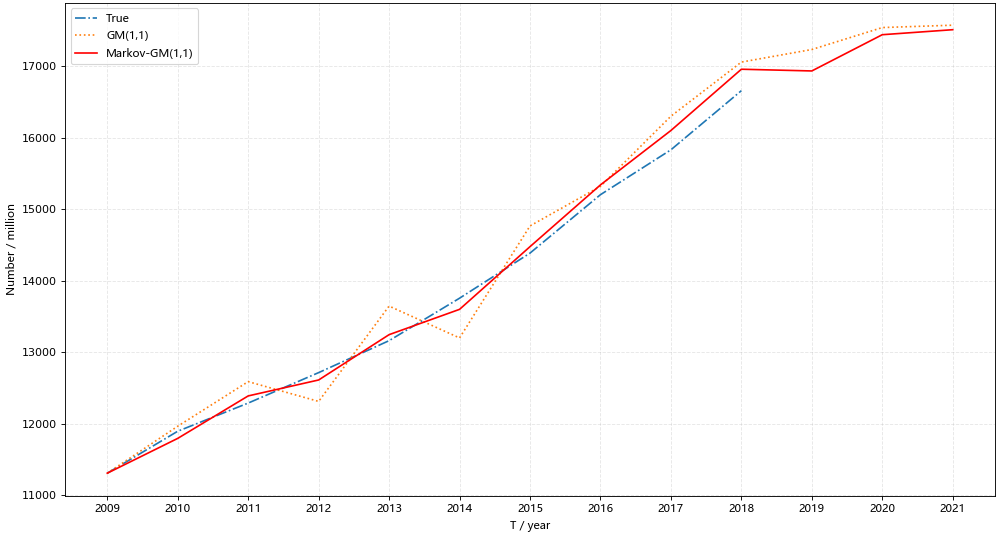
\includegraphics[width=1\textwidth]{pic/Figure_1.png}
	\caption{Comparison curve of prediction value of the number of the elderly}\label{afd}
\end{figure}


Similarly, the calculation of the medical demand forecast value for 2009-2018 is obtained as follows:
\begin{gather}
\widehat{X}(k+1)=258.7846e^{-0.043809k}-246.9258,k=1,2,\cdots,10
\end{gather}



The error status range is shown in the table ~\ref{ss}~.
\begin{table}[H]
	\centering\caption{Medical demand status interval division}\label{ss}
	\begin{tabular}{cccc}
		\toprule[1.5pt]
		{\centering Status}
		& {\centering $E_{1}$}
		& {\centering $E_{2}$}
		& {\centering $E_{3}$}
		\\
		\midrule[0.5pt]
		Residual interval &  $[-164.45,-58.74]$  &$(-58.74,58.74]$ & $(58.74,164.45]$  \\ 
		\bottomrule[1.5pt]	
	\end{tabular}
\end{table}

The medical demand forecast is classified into the error interval as shown in the table ~\ref{Hss}~.
\begin{table}[H]
	\centering\caption{Medical demand error status interval}\label{sss}
	\begin{tabular}{ccccccccccc}
	\toprule[1.5pt]
	{\centering year}
	& {\centering 2009}
	&{\centering 2010}
	& {\centering 2011}
	&{\centering 2012}
	& {\centering 2013}
	& {\centering 2014}
	&{\centering 2015}
	&{\centering 2016}
	&{\centering 2017}
	&{\centering 2018}
	\\
	\midrule[0.5pt]
	Residual interval &  $E_{2}$  &$E_{3}$ & $E_{1}$&$E_{2}$ &$E_{3}$ &$E_{1}$&$E_{1}$&$E_{3}$&$E_{2}$&$E_{2}$\\ 
	\bottomrule[1.5pt]	
\end{tabular}
\end{table}

From this, the initial state probability vector $t_{0}$ is obtained, and the transfer matrix $P$ is:
\begin{gather}
\begin{matrix}
t_{0}'=[3/10,2/5,3/10]\\ 
\\ 
P'=\left(\begin{array}{lll} 0 & 1/2 & 1/2\\ 1/8 & 3/4 & 1/8 \\1/2 & 1/2 & 0\end{array}\right)
\end{matrix}
\end{gather}

The predicted solution obtained by gray prediction and Markov correction is shown in the figure ~\ref{asf}~.
\begin{figure}[H]
	\centering
	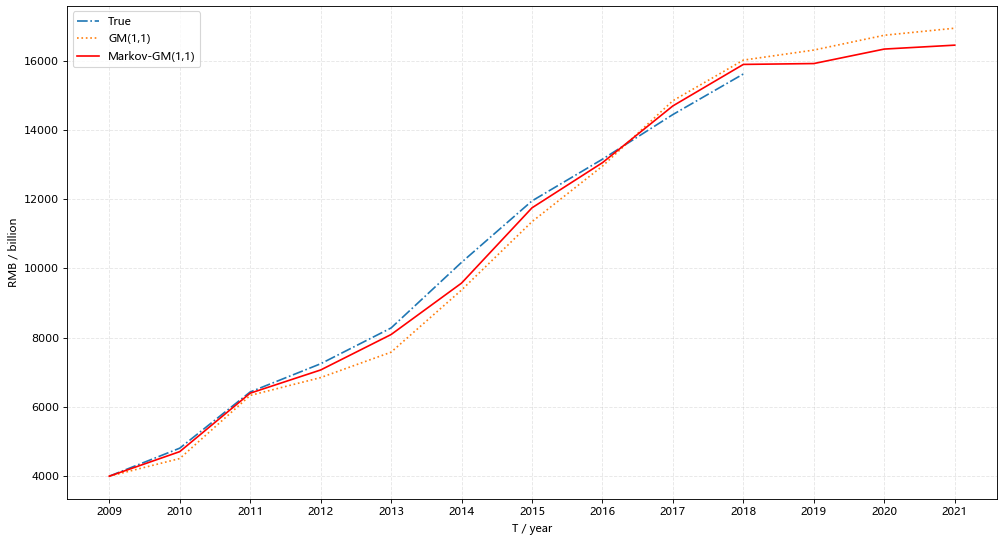
\includegraphics[width=\textwidth]{pic/Figure_2.png}
	\caption{Comparison curve of medical demand forecast}\label{asf}
\end{figure}


\subsubsection{Conclusion}

According to the direct comparison of the prediction solution curves in Figure ~\ref{afd}~ and figure ~\ref{asf}~, the predicted value corrected by Markov model has higher fitting degree and consistent volatility compared with the traditional gray prediction value, and can reflect the actual value fluctuation better than the traditional gray model prediction value. The prediction indexes of the two models are shown in table ~\ref{jjj}~:

 \begin{table}[H]
	\centering\caption{Test of prediction results}\label{jjj}
	\begin{tabular}{cccc}
		\toprule[1.5pt]
		{\centering Test parameters}
		&{\centering RMSE}
		&{\centering MAPE}
		&{\centering NSE}
		\\
		\midrule[0.5pt]	
		GM(1,1) for elderly people&   3040.04 &  0.0213 & 0.9455\\ 
		Markov-GM(1,1) for elderly people&  1238.64  &  0.0095  &  0.9900 \\ 
		GM(1,1) for medical demand&  265.88   & 0.0628   &0.8178  \\
		Markov-GM(1,1) for medical demand &   101.13 &   0.0273 & 0.9736  \\   
		\bottomrule[1.5pt]	
	\end{tabular}
\end{table} 

From the above prediction results, it can be concluded that the RMSE of the number of patients and the number of deaths calculated by using the modified grey Markov model is smaller than that of the traditional grey model, which shows that the modified results are more reliable. The MPAE value of the modified model is closer to $0 $and the NSE value is closer to $1 $compared with the traditional model, which shows that the improved gray Markov model has a higher fitting degree and better prediction effect, which is suitable for the short-term prediction of the number of infectious diseases and deaths.


	  \subsection{The model of Problem 2}
	\subsubsection{Establishment of model}  
According to the different data of each year,we modified the grey markov model of the first question.

	  \begin{gather}
\left\{\begin{matrix}
\overline{x}(k) =\widehat{x}(k)-\eta\\
\widehat{X}(k+1)=[X^{(0)}(1)-\frac{u}{a}]e^{-ak}+\frac{u}{a},k=1,2,\cdots,13\\ 
\eta =\begin{bmatrix}
p_{E1} & p_{E2} & p_{E3}
\end{bmatrix} \cdot \begin{bmatrix}
\overline{E}_{1} & \overline{E}_{2} & \overline{E}_{3}
\end{bmatrix}^{T}
\end{matrix}\right.
\end{gather}

The revised predicted number of patients in year $k$ was  $\overline{x}(k)$ , $\widehat{x}(k)$ is the traditional predicted value of  $GM(1,1) $, $\eta$ is the expected error of $GM$ in year$ k$.

	     \subsubsection{Calculation of predictors}
We set $X_{i}$ as the incidence data of 13 diseases from 2009 to 2021 in hubei province, $X_{i}=[x_{i1},x_{i2},x_{i3},x_{i4},x_{i5}](i=1,2,\cdots,13)$, The prediction results are obtained by using markov model. Similarly, Put the death toll data $X_{i}'=[x_{i1}',x_{i2}',x_{i3}',x_{i4}',x_{i5}'](i=1,2,\cdots,13)$ into the forecasting results $X_{i}'=[x_{i1}',x_{i2}',x_{i3}',x_{i4}',x_{i5}',x_{i6}'](i=1,2,\cdots,13)$. 

According to the prediction, the growth rate of the number of cases, the growth rate of the number of deaths and the mortality rate of the sick population in 2019 are respectively:

 \begin{gather}
\left\{\begin{matrix}
\delta _{i}=\frac{x_{i6}-x_{i5}}{x_{i5}} \times 100\%\\ 
\delta '_{i} =\frac{x_{i6}'-x_{i5}'}{x_{i5}'} \times 100\%\\ 
\eta_{i} =\frac{x_{i6}'}{x_{i6}} \times 100\%
\end{matrix}\right.
\end{gather}


Get the decision attribute vector of each group:

\begin{gather*}
d_{i}=[x_{i6},x_{i6}', \delta_{i} , \delta _{i}',\eta_{i} ]
\end{gather*}


Similarly, the number of morbidity and mortality of various diseases in Hubei province were brought into the model to obtain the decision attribute vectors of various diseases $d_{i}'(i=1,2,\cdots,13)$.

\subsubsection{TOPSIS}


Let the disease multi-attribute decision matrix $A=(a_{ij})_{13 \times 5}$ be expressed as:

  \begin{gather*}
A= [d_{1}^{T},d_{2}^{T},\cdot,,d_{13}^{T}]^{T}
\end{gather*}

Normalize $A$ to obtain normalized decision matrix$B=(b_{ij})_{13 \times 5}$, where:

\begin{gather*}
b_{ij}=a_{ij}/\sqrt{\sum_{i=1}^{13}a_{ij}^{2}},i=1,2,\cdots,13;j=1,2,\cdots,5
\end{gather*}


It is assumed that regions with high growth rates of the number of patients and deaths need to focus on prevention and control,  construct weight vectors:


 \begin{gather}
W=[0.15,0.3,0.15,0.3,0.1]
\end{gather}

The weighted canonical matrix, positive ideal solution,  negative ideal solutioncan be obtained as follows: $C=(c_{ij})_{13 \times 5}$,  $C^{*}=[c_{1}^{*},c_{2}^{*},c_{3}^{*},c_{4}^{*},c_{5}^{*}]$,  $C^{0}=[c_{1}^{0},c_{2}^{0},c_{3}^{0},c_{4}^{0},c_{5}^{0}]$,  where in:
     
     \begin{gather*}
\left\{\begin{matrix}
c_{ij}=w_{j} \cdot b_{ij} ,i=1,2,\cdots,13;j=1,2,\cdots,5\\
c_{j}^{*}=\underset{i}{max}(c_{ij}) ,j=1,2,\cdots,5\\
c_{j}^{0}=\underset{i}{min}(c_{ij}) ,j=1,2,\cdots,5
\end{matrix}\right.
\end{gather*}

Calculating the distance from each disease attribute decision vector to the positive and negative ideal solution. The distance from      $d_{i}$ to the positive ideal solution and from $d_{i}$ to the negative ideal solution is: 

\begin{gather*}
\left\{\begin{matrix}
s_{j}^{*}=\sqrt{\sum_{j=1}^{n}(c_{ij}-c_{j}^*)^{2}},i=1,2,\cdots,13\\
s_{j}^{0}=\sqrt{\sum_{j=1}^{n}(c_{ij}-c_{j}^{0})^{2}},i=1,2,\cdots,13
\end{matrix}\right.
\end{gather*}

Calculating the comprehensive evaluation index of each program:
 \begin{gather}
f_{i}^{*}=s_{j}^{0}/(s_{j}^{0}+s_{j}^{*}),i=1,2,\cdots,13
\end{gather}

Obtain the order of key prevention and control diseases according to  $f_{i}^{*}$ (range from large to small). Similarly, the decision vector $d_{i}'(i=1,2,\cdots,13)$ of each disease can be brought into TOPSIS model to obtain the priority of disease prevention and control


\subsubsection{Results and Conclusion}

The number of cases and deaths of each occupation were put into the grayscale markov model to obtain the predicted values, as shown in table ~\ref{zhdsaiye1}~ .



 \begin{table}[H]
	\centering\caption{Predicted results of patients with various diseases}\label{zhdsaiye1}
	\begin{tabular}{ccccccc}
		\toprule[1.5pt]
		{\centering disease/10*thousand}
		& {\centering 2009}
		& {\centering 2010}
		& {\centering $\cdots$}
		& {\centering 2019}
		& {\centering 2020}
		& {\centering 2021}
		\\
		\midrule[0.5pt]	
		Immunodeficiency &   1.5686& 1.5021&	$\cdots$ &	1.3377
		  & 1.2777& 1.2673\\ 
		Endocrine disease&  20.3322 &  18.129 &	$\cdots$ &20.3322
		  &	19.2462&18.6414\\ 
		Nervous system&  6.8927& 5.8433 &		$\cdots$  &	8.6325 &	8.9582&7.8506\\
		Urogenital diseases&7.3363
		& 7.2032
		&		$\cdots$  &6.892
		&6.943
		&7.042
		\\
		$\cdots$ &  $\cdots$ &  $\cdots$&  $\cdots$&  $\cdots$&  $\cdots$&  $\cdots$   \\   
		Heart disease  & 128.8231
		& 129.1872
		&$\cdots$ 
		&149.45
		&153.454
		&155.6778
		 \\ 
		infectious disease & 7.9431
		 &7.421
		 &$\cdots$
		  &5.437
		  &	4.824
		  &	4.534
		   \\
		   Perinatal diseases
		   & 1.5351 &2.0284 &$\cdots$
		   &1.124 &0.943  &0.7423 \\
		   
		    Digestive system diseases
		   & 16.578
		   
		   &16.9643
		   
		   &$\cdots$
		   &14.45
		   
		   &14.43
		   
		   
		   &14.34
		   
		   \\
		   Other
		   & 10.7305
		   
		   
		   &9.5811
		   
		   
		   &$\cdots$
		   &6.745
		   
		   
		   &7.345
		   
		   
		   &7.123
		   
		   \\
		\bottomrule[1.5pt]	
	\end{tabular}
\end{table}

Calculate the positive ideal solution and the negative ideal solution as:
\begin{gather*}
\begin{matrix}
C^{0}=[0.0066,0.0048,0.0653,0.0261,0.0331]\\
C^{*}=[-0.1856,-0.1847,-0.0809,-0.1163,-0.0929]
\end{matrix}
\end{gather*}

~\\

That is, the comprehensive evaluation index of the disease of $13$ is shown in the figure ~\ref{oc}~:

  \begin{figure}[H]
  	\centering
  	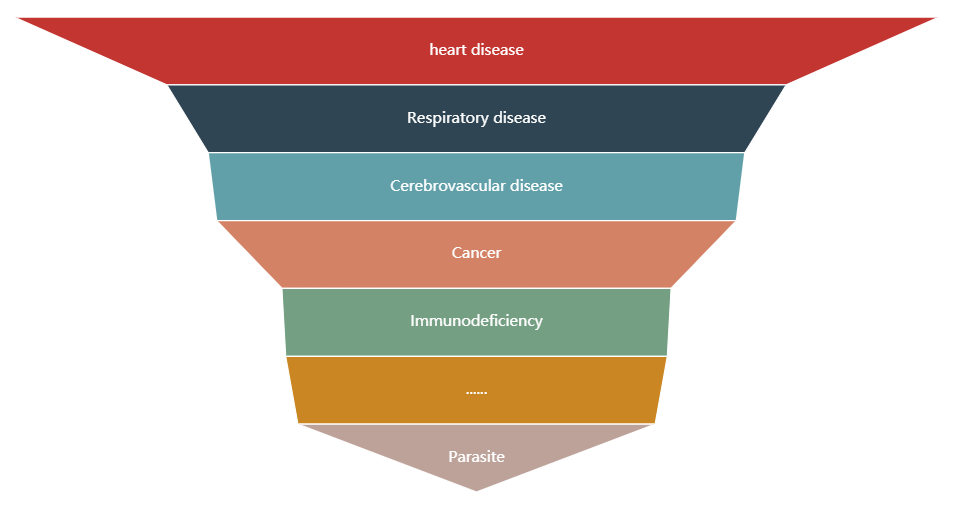
\includegraphics[width=\textwidth]{pic/Figure_3.png}
  	\caption{TOPSIS scores for different diseases}\label{oc}
  \end{figure}


According to TOPSIS ranking, the number of heart attack and death in Hubei Province is on the rise, and the rising rate is high, which belongs to the key population of prevention and control.


  \begin{figure}[H]
	\centering
	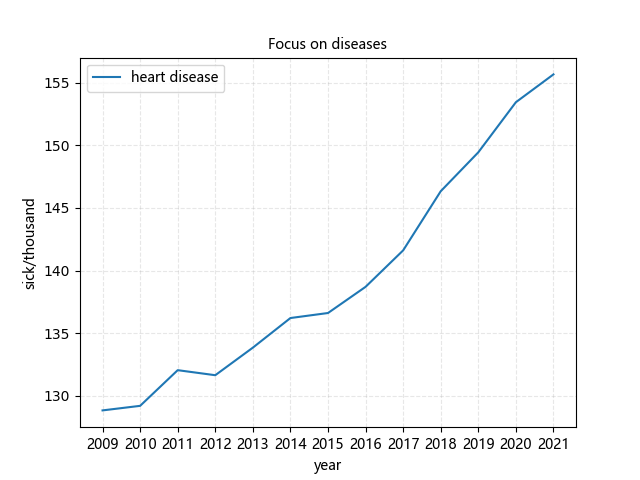
\includegraphics[width=\textwidth]{pic/Figure_4.png}
	\caption{Focus on diseases}\label{oc4}
\end{figure}


\subsection{The model of Problem 3}
	\subsubsection{Establishment of model}  
	 \paragraph{ $M/M/c/\infty$ model}
As the theory of $M/M/c/\infty$ illusteate:
\begin{gather}
\left\{\begin{array}{ll}{P_{0}=} & {\left[\sum_{k=0}^{-1} \frac{1}{k !}\left(\frac{\lambda}{\mu}\right)^{k}+\frac{1}{c !} \cdot \frac{1}{1-\rho} \cdot\left(\frac{\lambda}{\mu}\right)^{c}\right]^{-1}} \\ {P_{n}=} & {\left\{\begin{array}{ll}{\frac{1}{n !}\left(\frac{\lambda}{\mu}\right)^{n} P_{0}} & {(n \leqslant c)} \\ {\frac{1}{c ! c^{n-c}}\left(\frac{\lambda}{\mu}\right)^{n} P_{0}} & {(n>c)}\end{array}\right.}\end{array}\right.
\end{gather}
In the above expression, n is the amount of patient.$p_{n}$ is the probability of number of patient reach n in the moment t. C represents the amount of doctors in an outpatient department. $\lambda$ means the average arrival rate of patients. And the $\mu$ means the average inspection rate of the doctor.

Based on this theory, the following relation is set up:       
\begin{gather}
\left\{\begin{array}{l}{L_{s}=L_{q}+\frac{\lambda}{\mu}} \\ {L_{q}=\sum_{n=c+1}^{\infty}(n-c) P_{n}=\frac{\left(c_{\rho}\right)^{c} \rho}{c !(1-\rho)^{2}} P_{0}}\end{array}\right.
\end{gather}
In the above expression, $L_{s}$ is the average length of the queuing which means the number of patient waiting in the system. Depending on it, we could derive the expression of average waiting time $W_{q}$ and average time of stay $W_{s}$:
\begin{gather}
\left\{\begin{matrix}W_{q}=\frac{L_{q}}{\lambda }
\\ W_{s}=\frac{L_{s}}{\lambda }
\end{matrix}\right.
\end{gather}
	\subsubsection{Solution of model}
\paragraph{Optimized systems design} 
For $M/M/c/\infty$ system, the expection of the social cost per hour in the steady state is set up as $Z$. And $Z$ could be calculated as the following expression:     
 \begin{gather}
 z=c_{s} \cdot c+c_{w} \cdot L_{s}
 \end{gather}
 In this expression, $C$ is the number of doctors in the outpatient department. $C_(s)$ represents the average hourly wage of the doctors while $C_(w)$ represents the patient's.$L_{s}$ is the amount of patient waiting in the system witch is function of $C$.Thus ,$Z$ is the function of $C$. To get the optimal solution of $C^*$ which make $Z$ the minimum, we adopt the marginal analysis to solve it.And accroding to the feature that $Z$ is the minimum, the following relation exists:  
\begin{gather}
\left\{\begin{matrix}Z(c^*)\leqslant Z(c^*-1)
\\ Z(c^*)\leqslant Z(c^*+1)
\end{matrix}\right.
\end{gather}
 Take expression (15) into expression (16) to gain:
  \begin{gather}
L(C^*)-L(C^*+1)\leqslant \frac{C_(s)}{C_(w)}\leqslant L(C^*-1)-L(C^*)
 \end{gather}
Thus, we utilize the ergodic algorithm to obtain the value of $C^*$.
\subsection{The model of Problem 4}

	\subsubsection{Establishment of model}  
\paragraph{Latent class analysis (LCA)}
we use latent class analysis (LCA) to identify distinct consumer segments in the hospital care markets based on detailed information on their use of hospital services. By examining the hospital utilisation pattern of each type, we assign putative names for all types. For indicators of hospital use, we consider not only the location and frequency of admissions, but also resource use during admissions, which reflects patient health. The indicators of resource use that we considered are the number of secondary procedures, which reflect the complexity of procedures for  example due to comorbidities, the length of stay and any record of emergency department  presentation. The resultant patient types are described in terms of their demographics and background characteristics, as well as variables that can be  manipulated such as income and lifestyle-related factors. And in the end, we exploit the availability of hospital data in the post-survey period to test the  relevance of the patient types in predicting future hospital utilisation. 

Let $Y_{i}=(Y_{i1},\cdots ,Y_{iM})$  denote patient's response to $M$ hospital indicator variables, where the possible values of $Y_{iM}$ are $1,\cdots ,r_{m}$. Let $L_{i}=1,2,\cdots ,n_{c}$be the latent type of patient. Where $n_{c}$ is the possible number of latent types.And let $X_{i}$ denote the covariates of patient $i$ that affects the market segmentation.The contribution by patient $i$ to the likelihood is:

\begin{gather}\label{sda}
\text { (1) } P\left(Y_{i}=y | X_{i}=x\right)=\sum_{l=1}^{n_{c}} \gamma_{l}(x) \prod_{m=1}^{M} \prod_{k=1}^{r_{m}} \rho_{m k | l}^{I\left(y_{m}=k\right)}
\end{gather}
where $I(y_{m}=k)$ is an indicator function that is equal to $1$ if $y_{m}$ is equal to $k$ and $0$ otherwise. The parameters to estimate are the probability of membership in each latent
type, which is the gamma parameters, $\gamma$ , and the item-response probabilities conditional on
type membership, which is the rho parameter, $\beta$. The gamma parameter can be given by a
multinomial logit (MNL) model such as:
\begin{gather}
\gamma_{l}(x)=P\left(L_{i}=l | X_{i}=x\right)=\frac{\exp \left(x \beta_{l}\right)}{\sum_{j=1}^{n_{c}} \exp \left(x \beta_{j}\right)^{\prime}}
\end{gather}
where $\beta$ is the MNL coefficient.
\subsubsection{Solution of model}
From ~\ref{sda}~, we can see that the model will increase in size very quickly with $M$ and $r_{m}$. For example, a model with eight binary indicators would result in 28 or 256 cells. In our case, we have six hospital indicator variables which are a mix of continuous and count variables at many levels. Therefore, some grouping of the levels is needed. We base ours on the
inspection of the distribution of each indicator with the intention that each level represents
a distinct case of hospital use. 

The next part of our analysis concerns the extent to which the identified patient types can
predict future demand for hospital services. The patient types are included as covariates, and the identifying	restriction is satisfied using lifestyle variables; lifestyles affect the probability of an admission but do not directly affect the choice between public or private hospital. We us	hospital data from a year after the survey date. Because only a few patients in our data were hospitalised for the same health problems again in the following year, for prospective	use, we consider both repeat procedures and the overall demand for any procedure.In this case, we find that private health insurance can lower the utilisation of public hospitals, thereby reducing the public health care burden. A reduction in health costs may	also be achieved through public policies that promote a general improvement in health to
reduce use of resources per admission. 

As a consequence, the strategies is to moderate the private health insurance and encourage the private hospital to establish the outpatient department the public hospital have little of while improving the quality of service of private hospital.



\subsection{A letter to the medical department}

\textbf{Dear Medical leaders}:
  ~\\


According to our modeling research, the aging trend in China is increasingly strengthened, and the majority of people's medical needs are increasingly high. It is estimated that the aging population over 65 will reach 170 million in 2021, which means that China will enter the aging society. According to the data, China's aging is on the rise, and meeting the medical and old-age needs of the elderly will be a huge social problem. Therefore, we should take measures as soon as possible in the field of gerontology scientific research, clinical medicine, rehabilitation nursing and public health policy, health management to actively carry out the diagnosis and treatment of the elderly related diseases difficult critical illness, demonstration and promotion of appropriate and effective high-level diagnosis and treatment technology; We will carry out teaching and training of high-level geriatric medical personnel, and train backbone clinical technicians and academic leaders. Undertake national geriatric medicine clinical translational research, in view of the elderly health has a major impact on disease organizations to carry out the relevant scientific research, in a timely manner to translate into clinical application and scientific research achievements at home and abroad for the next "five-year plan", and establish a medical, nursing, scientific research, teaching, prevention, management and policy making of the "seven" function of the major disease prevention and health management at the core of the organization.

Strengthening cooperation between public and private hospitals is the focus of improving medical efficiency. In order to alleviate the "three difficulties" of patients in public hospitals, such as difficulty in seeing a doctor, difficulty in hospitalization and difficulty in operation, public hospitals and private hospitals can cooperate and learn from each other. The cooperation between public hospitals and private hospitals includes public hospitals exporting management and technology to private hospitals, public hospitals borrowing beds from private hospitals, public hospitals hosting private hospitals, private hospitals or private capital participating in public hospitals. The cooperative hospital carries out standardized management and operation according to the standards of public hospitals to provide medical services for ordinary patients. At the same time, public hospitals' technical advantages, talent advantages and management advantages are utilized to enhance the popularity and credibility of private hospitals, improve the management and technical level of private hospitals, and create a win-win situation for public hospitals, private hospitals, patients and the society. It is suggested to set up a hospital management group with large public hospitals as the leading role to promote the development of private hospitals or small hospitals and at the same time make rational use of resources.

Finally, according to the model in question 2, we can predict the key disease prevention of each province in the next few years, and the corresponding province can take emergency measures on the medical problems that should be solved most, strengthen the prevention and treatment of related diseases, establish an appropriate medical insurance system, and the corresponding hospital should also make preparations in advance. I believe that with the hard work of all medical staff, China's medical environment will be better and better.

This is for your reference only.

%====================================\input{StrengthsandWeaknesses}============================================
\section{Strengths and Weaknesses}

\subsection{Strengths}
\begin{enumerate}
\item The gray prediction value improved by Markov model has higher fitting degree with the actual value, and the volatility is consistent, so the prediction effect is better
\item the queue model of more service system based on the analysis of queue Doctor-patient system with the method of queueing theory.
\end{enumerate}

\subsection{Weaknesses}
\begin{enumerate}
\item The GM(1,1) prediction model can only make short-term prediction, and is not suitable for long-term prediction.
\item Effective coefficient of restitution can not be calculated accurately.This affect the accuracy of the result of the model.
\end{enumerate}

\section{Conclusion}
%========================Bibtex
\newpage
	\nocite{*}		%??????????
%\bibliography{wenxian.bib}
%	%???????wenxian.bib?????
%	
\begin{thebibliography}{9}%??9
	\bibitem{bib:one}Javed S A, Liu S, Mahmoudi A, et al. Patients' satisfaction and public and private sectors' health care service quality in Pakistan: Application of grey decision analysis approaches[J]. The International journal of health planning and management, 2019, 34(1): e168-e182.
	
	\bibitem{bib:2}Xu S, Zou B, Shafi S, et al. A hybrid Grey-Markov/LUR model for PM10 concentration prediction under future urban scenarios[J]. Atmospheric environment, 2018, 187: 401-409.
	
	\bibitem{bib:3}Ye J, Dang Y, Li B. Grey-Markov prediction model based on background value optimization and central-point triangular whitenization weight function[J]. Communications in Nonlinear Science and Numerical Simulation, 2018, 54: 320-330.
	
	\bibitem{bib:4}Saad Ahmed Javed,Sifeng Liu. Correction to: Predicting the research output/growth of selected countries: application of Even GM (1, 1) and NDGM models[J]. Scientometrics,2019,120(3).
	
	\bibitem{bib:5}Ervural B C, Zaim S, Demirel O F, et al. An ANP and fuzzy TOPSIS-based SWOT analysis for Turkey?s energy planning[J]. Renewable and Sustainable Energy Reviews, 2018, 82: 1538-1550.
	
	\bibitem{bib:6}Olson D L. Comparison of weights in TOPSIS models[J]. Mathematical and Computer Modelling, 2004, 40(7-8): 721-727.
	
	\bibitem{bib:7}Gu M, Johar M. Profiling hospital utilization in a mixed public?private system[J]. Applied Economics, 2017, 49(4): 361-375.
	
	\bibitem{bib:8}Alnowibet K, Tadj L. Analysis of Two Phases Queue With Vacations and Breakdowns Under T-Policy[M]//Advanced Methodologies and Technologies in Digital Marketing and Entrepreneurship. IGI Global, 2019: 13-31.
	
	\bibitem{bib:9}Liao J, Mawditt C, Scholes S, et al. Similarities and Differences in Health-Related Behaviour Clustering Among Older Adults in East and West: A Latent Class Analysis of Global Ageing Cohorts[J]. Available at SSRN 3218733, 2018.
	
	
\end{thebibliography}

\newpage
%??
%\appendix %%??

\end{document}
